\documentclass[xcolor=svgnames,dvipsnames,table, hyperref=pdftex, mathserif, presentation]{beamer}
\usepackage{amsmath,amssymb,amsfonts,amsthm}
\usepackage{ctex}
\usepackage{graphics}
\usepackage{graphicx}
\usepackage{xcolor}
\usepackage{wasysym}
\usepackage{bbm}
\usepackage{url}
\usepackage{beamerleanprogress}
\usepackage{tikz-dependency}
\usepackage{tikz-qtree}
\usepackage{multirow}

\newcommand{\tabincell}[2]{\begin{tabular}{@{}#1@{}}#2\end{tabular}}%放在导言区
\usetheme{CambridgeUS}
%\usetheme{Pittsburgh}
\usecolortheme{orchid} % seahorse  orchid rose
\setbeamertemplate{blocks}[rounded][shadow=true]
\AtBeginSection[]{%
  \begin{frame}<beamer>
    \frametitle{Outline}
      \tableofcontents[current] 
    \end{frame}
  \addtocounter{framenumber}{-1}% If you don't want them to affect the slide number
}
\AtBeginSubsection[]
{
  \begin{frame}
  \frametitle{Outline}
    \tableofcontents[currentsection,currentsubsection]
  %\tableofcontents[sectionstyle=show/hide,subsectionstyle=hide/show/hide]
  \end{frame}
  \addtocounter{framenumber}{-1}% If you don't want them to affect the slide number
}
\newcommand{\setof}[1]{\ensuremath{\left \{ #1 \right \}}}
\newcommand{\tuple}[1]{\ensuremath{\left \langle #1 \right \rangle }}
\newcommand{\red}[1]{\textcolor{red}{#1}}
\newcommand{\brown}[1]{\textcolor{brown}{#1}}
\newcommand{\green}[1]{\textcolor{green}{#1}}
\newcommand{\blue}[1]{\textcolor{blue}{#1}}
\newcommand{\cyan}[1]{\textcolor{cyan}{#1}}

%gets rid of navigation symbols
\setbeamertemplate{navigation symbols}{}

\begin{document}

\title[RNN]{Sentence representation \\ via Recursive Nerual Networks}

\institute[icst@pku]{
  
}
\author[Zhe Han]{\\ Zhe Han \\  iampkuhz@gmail.com
}

\frame[t,plain]{ \titlepage } % [t,plain]

\frame{
  \frametitle{ Outline  }
  
   \begin{itemize}

  \item 3个表示句子向量的模型
    \begin{itemize}
      \item (展开的)递归自编码机解决复述问题 (2011NIPS)
      \item 递归自编码机+解决情感分析问题 (2011EMNLP)
      \item 基于语义依存树构建的递归神经网络解决图像描述问题 (2014TACL)
    \end{itemize}

  \item 不同句子向量模型的分析比较
    \begin{itemize}
    \item 穿插在模型介绍中
    \end{itemize}
  \end{itemize}
  
  \begin{block}{socher's paper: www.socher.org}
  \begin{itemize}
   \item \begin{footnotesize}
          Dynamic pooling and unfolding recursive autoencoders for paraphrase detection %(2011NIPS)
         \end{footnotesize}

   \item \begin{footnotesize}
          Semi-Supervised Recursive Autoencoders for Predicting Sentiment Distributions%(2011EMNLP)
         \end{footnotesize}

   \item \begin{footnotesize}
          Grounded Compositional Semantics for Finding and Describing Images with Sentences%(2014TACL)
         \end{footnotesize}

  \end{itemize}
  \end{block}

}

\frame{
  \frametitle{socher}
     \begin{figure}[h]
  \centering
  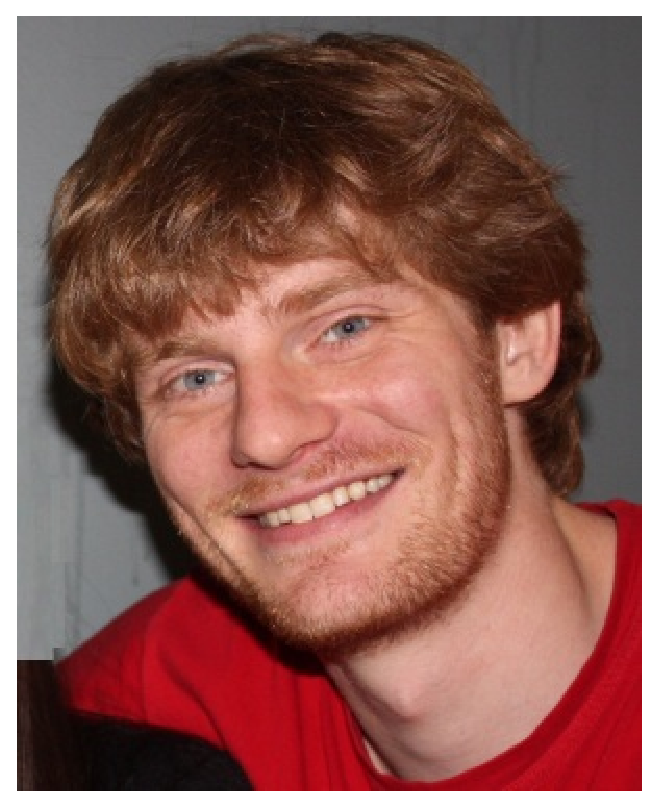
\includegraphics[width=0.15\textwidth]{RichardSocher}
  \end{figure}
  
  \begin{itemize}
   \item stanford毕业的博士
      \begin{itemize}
       \item  Chris Manning 和Andrew Ng的学生, 创业公司MetaMind的CTO
      \end{itemize}

  
    \item 此人非常喜欢用递归神经网络(Recursive Nerual Network)
	\begin{itemize}
	 \item 罗炳峰: 2014NIPS Global Belief Recursive Neural Networks
	\end{itemize}

  \end{itemize}

}

\frame{
    \frametitle{Motivation}
     \begin{itemize}
      \item 为什么要表示句子的语义向量
	  \begin{itemize}
	   \item 单词的语义向量以及有比较好的表示了(word2vec)
	   \item 中文维基百科谓词归一
	  
     \begin{figure}[h]
  \centering
  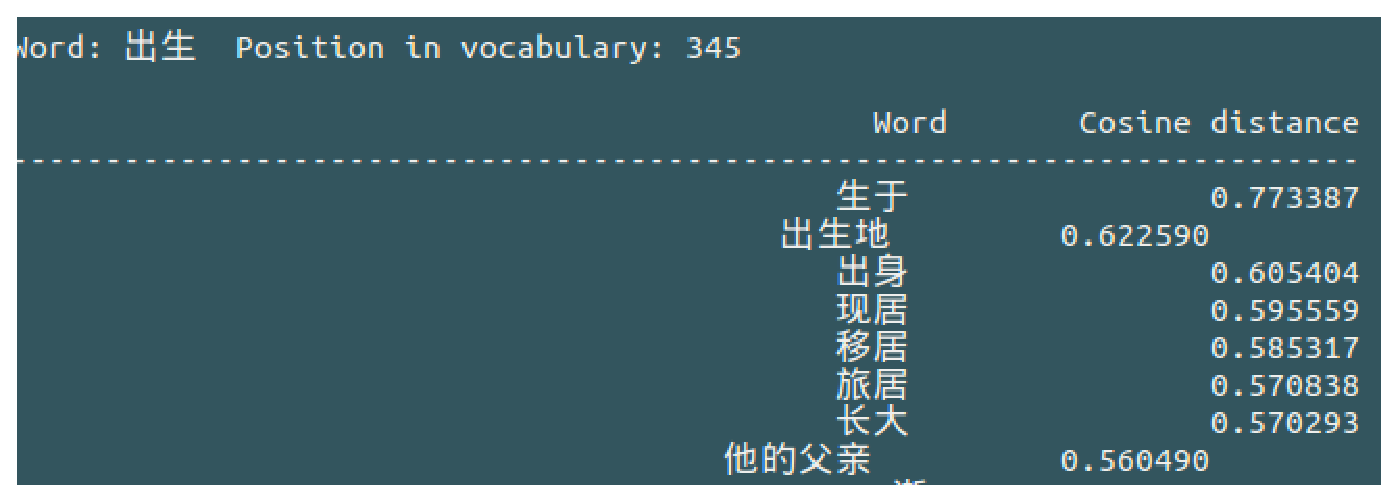
\includegraphics[width=0.75\textwidth]{word2vec1}
  \end{figure}
     \begin{figure}[h]
  \centering
  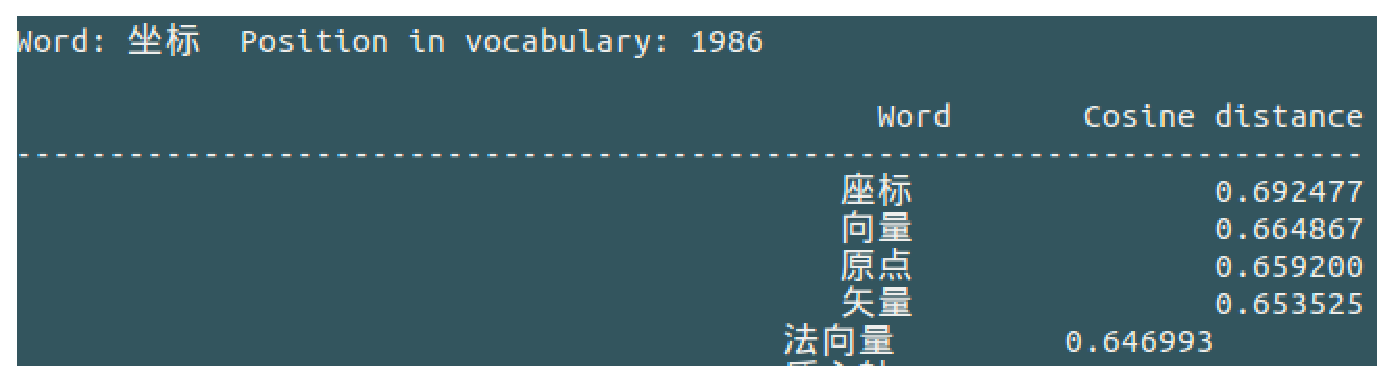
\includegraphics[width=0.75\textwidth]{word2vec2}
  \end{figure}
  
	  \end{itemize}

     \end{itemize}

}


\frame{
    \frametitle{Motivation}
     \begin{itemize}
      \item 为什么要表示句子的语义向量
	  \begin{itemize}
	   \item 单词的语义向量以及有比较好的表示了(word2vec)
	   \item 中文维基百科谓词归一
	      \begin{itemize}
	       \item 1500/16000 谓词含有word2vec向量, 其余为低频词或组合词
	      \end{itemize}
	  \item 利用客体的语义信息提取特征
	      \begin{itemize}
	       \item 客体一般是短语or句子, 需要从词向量提取短语向量
	      \end{itemize}

  
	  \end{itemize}

     \end{itemize}

}

\frame{
    \centering
    \begin{Large}
     复述检测
    \end{Large}


  \begin{block}{socher 2011NIPS}
  \begin{itemize}
   \item \begin{footnotesize}
          Dynamic pooling and unfolding recursive autoencoders for paraphrase detection %(2011NIPS)
         \end{footnotesize}
  \end{itemize}
  \end{block}
}

\frame{
  \frametitle{Paraphrase identification}
  
  \begin{itemize}
   \item definition
      \begin{itemize}
       \item 给定一组句子, 判断其是否是复述
	  \begin{itemize}
	   \item binary classification
	  \end{itemize}

      \end{itemize}
      
    \item Microsoft Research Paraphrase Corpus (MSRP)
	\begin{itemize}
	 \item train: 4,076 sentence pairs (2,753 positive: 67.5 \%)
	 \item test: 1,725 sentence pairs (1,147 positive: 66.5 \%)
	 \item 2个标注者, 83\%的一致性, 第三个人更正
	\begin{block}{Sample data}
	 \begin{itemize}
	 	 \item Sentence 1: Amrozi accused his brother, whom he called "the witness", of deliberately distorting his evidence.
	       \item Sentence 2: Referring to him as only "the witness", Amrozi accused his brother of deliberately distorting his evidence.
	       \item Class: 1 (true paraphrase)
	 \end{itemize}
	\end{block}
	
	\end{itemize}
  \end{itemize}

}


\frame{
    \frametitle{Paraphrase identification}
    \begin{itemize}
     \item 常用方法
	\begin{itemize}
	  \item 提取词汇特征,语义特征
	      \begin{itemize}
	       \item n-gram features, skip-gram fatures; POS tag, wordnet similarity, dependency tree relation, ...
	      \end{itemize}
	  \item SVM分类
	      \begin{itemize}
	       \item 或是投票分类
	      \end{itemize}
	\end{itemize}
    
    \item Challenge
	\begin{itemize}
	 \item 没有提取句子的全局信息( dependency features利用不足)
	 \item 对句子涵义的特征提取不足(没有真正理解句子)
	\end{itemize}

    \end{itemize}

}


\frame{
\begin{footnotesize}
    \frametitle{Paraphrase identification}
    \begin{block}{socher的方法}
	\begin{itemize}
	 \item 利用NYT新闻训练每个单词的向量(100维)
	 \item 对于每个句子(多个单词向量)采用训练一个递归的自动编码机, 得到一个句子级别的语义向量. 
	 \item 通过判断两个句子的语义向量的相似性得到语义相似性特征
	\end{itemize}
    \end{block}

    \begin{itemize}
	 \item 递归的自动编码机(Unfolding Recursive Autoencoder) 
	    \begin{itemize}
	     \item 抽取句子的语义向量, 得到语法数上每个节点(单词, 短语)的向量
	    \end{itemize}
	 \item Dynamic Pooling
	    \begin{itemize}
	     \item 对于长度变化的两个句子, 抽取固定维数的特征
	    \end{itemize}

	\end{itemize}
\end{footnotesize}
}
%

\frame{
\begin{footnotesize}
    \frametitle{Unfolding Recursive Autoencoder}
    \begin{itemize}
     \item Autoencoder
	\begin{itemize}
	 \item 希望压缩的特征(L2层)能表示原数据(L1层)
	    \begin{itemize}
	     \item 能表示等价于可以还原(L3层向量约等于L1层向量)
	    \end{itemize}

	\end{itemize}

     \item Recursive Autoencoder
	\begin{itemize}
	    \item Autoencoder in recursive structure
	\begin{itemize}
     \item Pollack提出(1990)
     \item 词向量没有压缩: $(0,...,0,1,0,...,0)$
    \end{itemize}
    
	 \item \footnotesize{进一步的, 对于深层的网络(语法树), 递归使用同一个简单的Autoencoder}
	\end{itemize}
	
	
	\begin{figure}[H]
	 \begin{minipage}[h]{0.33\linewidth}
\centering
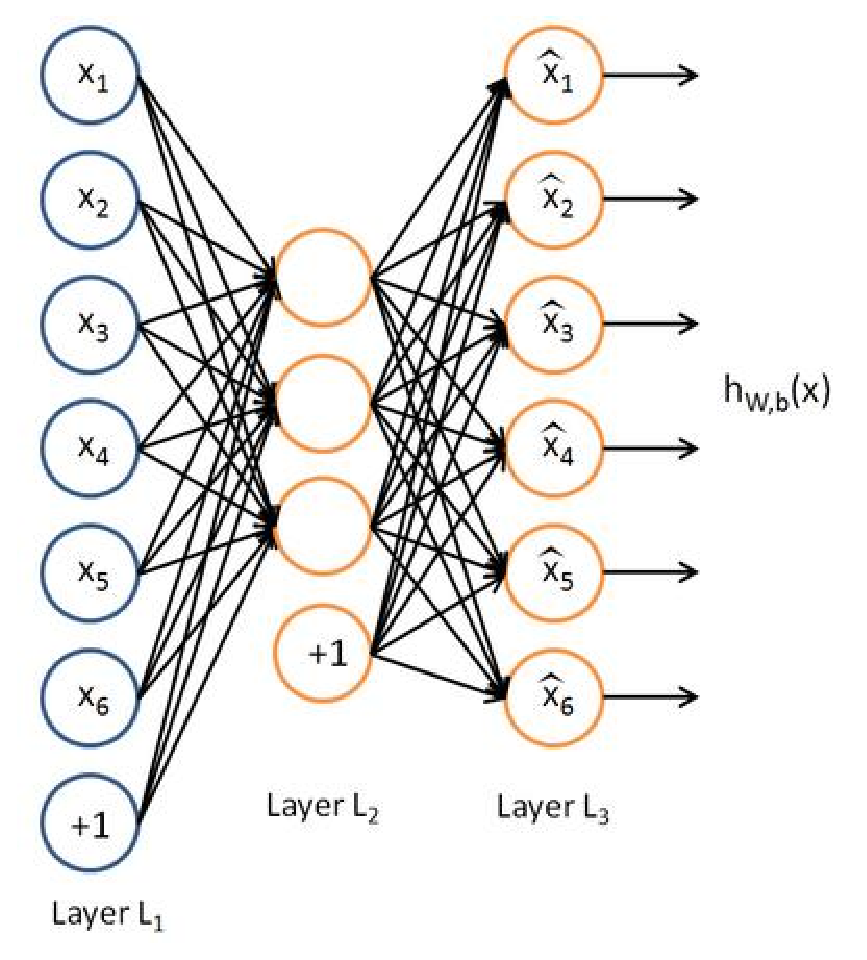
\includegraphics[width=0.8\textwidth]{Autoencoder.eps}
\end{minipage}
\begin{minipage}[h]{0.5\linewidth}
\centering
\includegraphics[width=0.9\linewidth]{RAE}

\end{minipage}
	\end{figure}
	
    \end{itemize}
\end{footnotesize}
}



\frame{
     \frametitle{Unfolding Recursive Autoencoder}
  \begin{figure}[h]
  \centering
  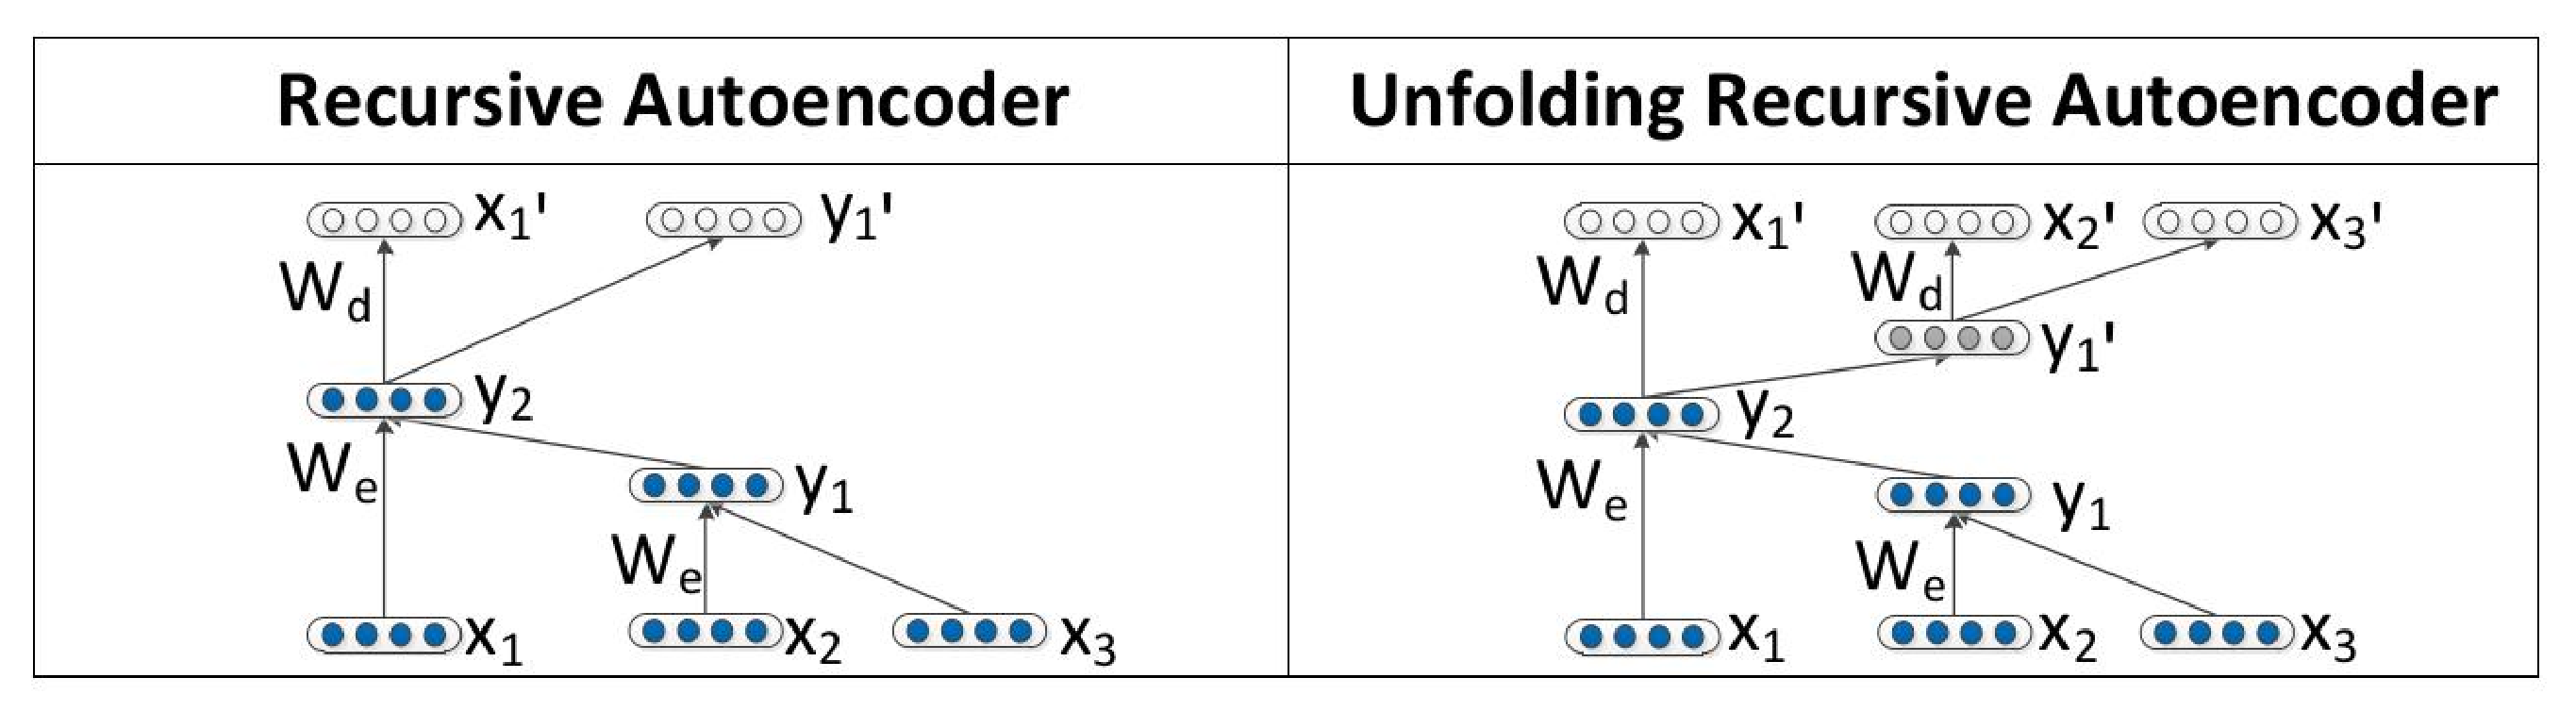
\includegraphics[width=0.8\textwidth]{uRAE}
  \end{figure}
  
  \begin{itemize}
      \item Recursive Autoencoder
      \item Comparison (on $y_2 -> x_1y_1$)
	  \begin{itemize}
	   \item Neural network
	      \begin{itemize}
	       \item minimum $\parallel y_2'-y_2\parallel$
	      \end{itemize}
	
	   \item Recursive Autoencoder
	   \begin{itemize}
	    \item minimum $\parallel[x_1';y_1']-[x_1;y_1]\parallel $
	   \end{itemize}
 
	   \item Unfolding Recursive Autoencoder
	      \begin{itemize}
	       \item  minimum $\parallel[x_1';x_2';...;x_j']-[x_1;x_2;...;x_j]\parallel $
	      \end{itemize}
	  \end{itemize}
      
    \end{itemize}
}


\frame{
  \frametitle{Dynamic Pooling(简要了解)}
  \begin{figure}[h]
  \centering
  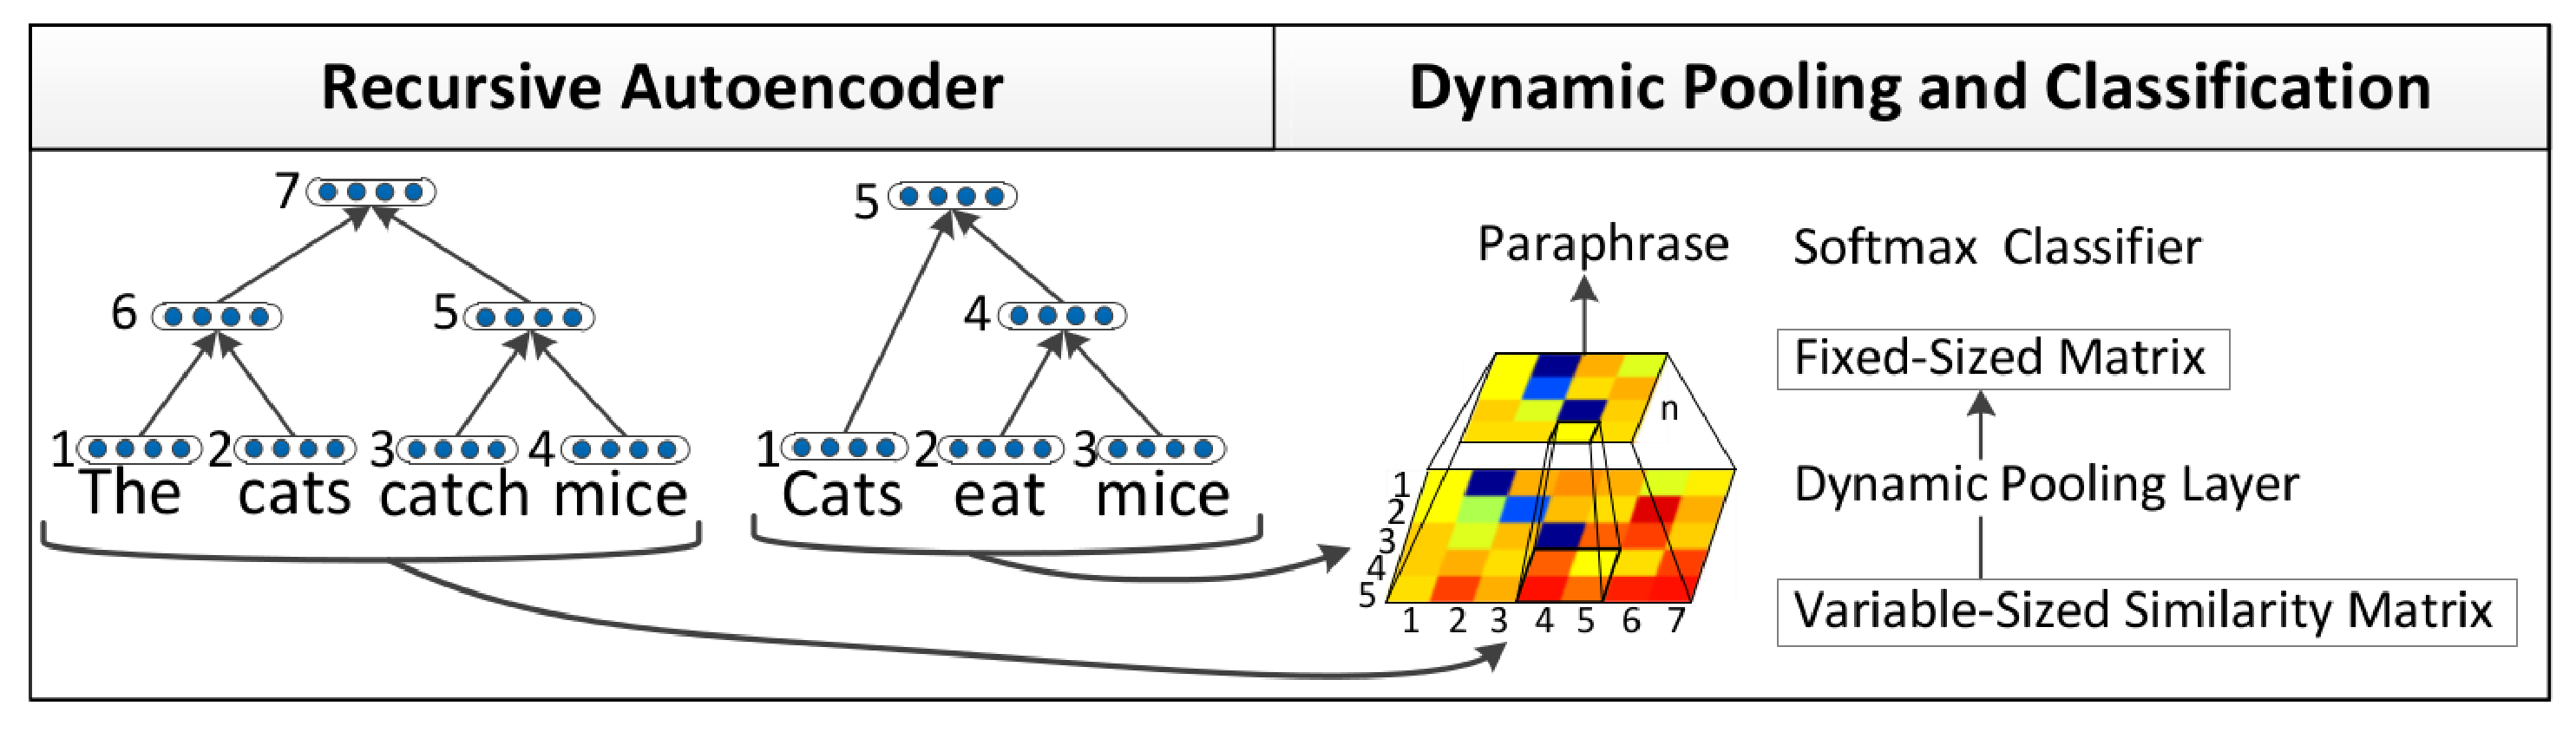
\includegraphics[width=0.8\textwidth]{DynamicPooling}
  \end{figure}
  
  
  \begin{itemize}
   \item motivation
      \begin{itemize}
       \item 如何对两个长度变化的句子抽取固定维数的特征?
       \begin{itemize}
        \item 长度为n的句子,cTree有(2n-1)个节点
       \end{itemize}

       \item 把不同长度的句子压缩(扩张)到相同的维数
      \end{itemize}
  \end{itemize}

  \begin{figure}[h]
  \centering
  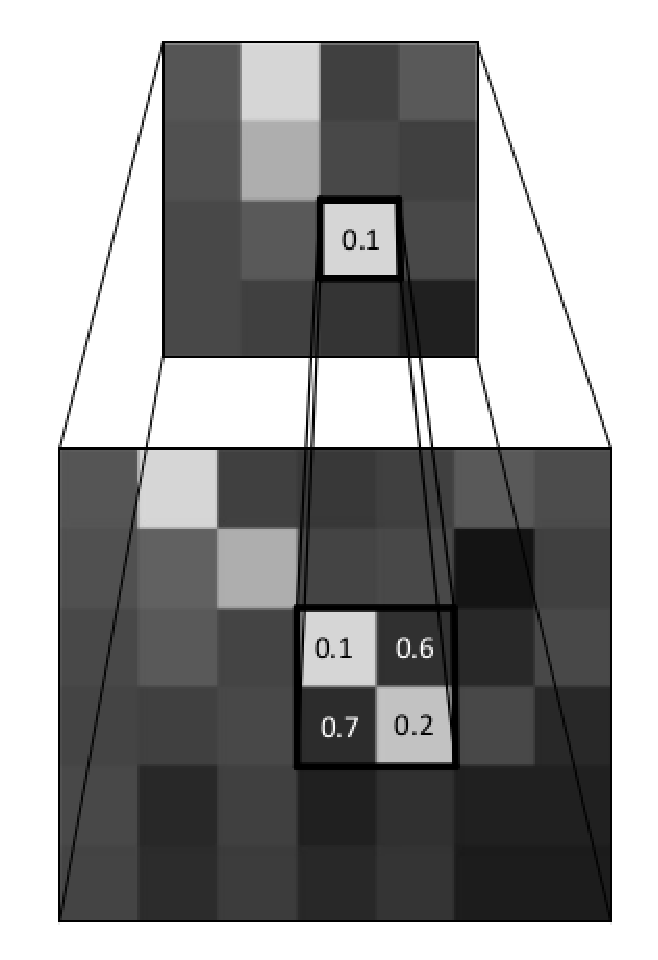
\includegraphics[height=0.4\textheight, angle=90]{pollingMin}
  \end{figure}

}

\frame{
  \frametitle{Paraphrase identification}
  \begin{itemize}
   \item QA
   \begin{itemize}
   \item 为何使用 uRAE 而不是 RAE 或者两个子节点的向量平均?
      \begin{itemize}
       \item 多个单词组成的句子/短语(高层节点),需要更多的单词信息,RAE只关心最近的2个儿子节点
       \item 向量平均:两个儿子向量的平均忽视了结构关系
       \item 实验证明,向量平均找不出来;RAE对2个单词组成的短语,识别其近义词效果很好;uRAE对于2-3个单词组成的短语的效果很好,甚至5个单词组成的短语有些也可以正确找到。
      \end{itemize}
      
  \begin{figure}
  \centering
  \includegraphics[width=0.65\textwidth]{Comp}
  \end{figure}
  \end{itemize}

  \end{itemize}

}



\frame{
    \centering
    \begin{Large}
     情感分析
    \end{Large}


  \begin{block}{socher 2011EMNLP}
  \begin{itemize}
   \item \begin{footnotesize}
          Semi-Supervised Recursive Autoencoders for Predicting Sentiment Distributions 
         \end{footnotesize}
  \end{itemize}
  \end{block}
}

\frame{
    \frametitle{Predicting Sentiment}
    \begin{itemize}
     \item identification
	\begin{itemize}
	 \item 给定一段话, 判断其情感极性(积极/消极, 正面评价/负面评价)
	 \item 给定一段话, 判断其评分分布(1-5颗星)
	\end{itemize}

    \item Experience project dataset(Potts, 2010)
	\begin{itemize}
	 \item 31,676个段子, 74,859条评分
	 \item 选取点评次数大于等于4次的段子
	 \end{itemize}
	 
	\begin{block}{Sample data}
  \begin{figure}
  \centering
  \includegraphics[width=0.95\textwidth]{EPData}
  \end{figure}
	\end{block}
	
    \end{itemize}

}

\frame{
    \frametitle{Predicting Sentiment}
  \begin{figure}
  \centering
  \includegraphics[width=0.3\textwidth]{UnsupervisedRAE}
  \end{figure}
  
    \begin{itemize}
     \item Unsupervised Recursive Autoencoder for Structure
	\begin{itemize}
	 \item 贪心的构造二叉树
	    \begin{itemize}
	     \item 每次计算当前状态任意一对相邻节点的合并代价, 取代价最小的一对合并, 直到结束
	     \item $p=f(W^{(1)}[c1:c2]+b^{(1)})$, $    [c_1':c_2']=W^{(2)}p+b^{(2)}$
	    \end{itemize}
	 
	 \item 考虑两个子节点的块大小
	    \begin{itemize}
	     \item 块越大越重要. 体现在重构误差中
	     \item $E_{rec}([c_1:c_2];\theta)=\frac{n_1}{n_1+n_2}\parallel c_1-c_1'\parallel^2+\frac{n_2}{n_1+n_2}\parallel c_2-c_2'\parallel^2$
	    \end{itemize}
	\end{itemize}

    \end{itemize}

}

\frame{
    \frametitle{Predicting Sentiment}
  \begin{figure}
  \centering
  \includegraphics[width=0.45\textwidth]{semiRAE}
  \end{figure}
  
    \begin{itemize}
     \item Semi-supervised Recursive Autoencoder for Structure
	\begin{itemize}
	 \item 扩展向量,加入情感分布向量d(维数为分类的个数)
	 \item 预测分布: $d(p;\theta)=softmax(W^{label}p)$
	 \item 真实分布: $t$
	 \item 采用交叉熵估计损失: $E_{cE}(p,t;\theta)=-\sum_{k=1}^{K}t_k\log d_k(p;\theta)$
	 \item 总体的损失函数为: $E([c_1:c_2]_s, p_s, t, \theta)=\alpha E_{rec}([c_1:c_2];\theta) + (1-\alpha)E_{cE}(p,t;\theta)$
	\end{itemize}

    \end{itemize}

}

\frame{
    \frametitle{Predicting Sentiment}
    
  \begin{itemize}
	 \item 对比之前的RNN模型
	    \begin{itemize}
	    \item 加入了情感分布特征
		\begin{itemize}
		\item 单纯的语言模型是不带情感极性的: good 和 bad词向量很像
		\end{itemize}
	    \item 没有使用句法树作为递归结构
		\begin{itemize}
		 \item 采用贪心的方法逐次向上递归
		 \item 句子的情感极性和句法结构并没有必然联系(情感性一般蕴含于修饰词)
		\end{itemize}

	    \end{itemize}
  
    \end{itemize}

}



\frame{
    \centering
    \begin{Large}
     理解图像描述问题
    \end{Large}


  \begin{block}{socher 2014TACL}
  \begin{itemize}
   \item \begin{footnotesize}
          Grounded Compositional Semantics for Finding and Describing Images with Sentences
         \end{footnotesize}
  \end{itemize}
  \end{block}
}


\frame{
  \frametitle{Finding and Describing Images with Sentences }
  
  \begin{itemize}
   \item definition
      \begin{itemize}
       \item 给定一段描述(一个句子), 找出其描述的图片
       \item 给定一张图片, 找出描述他的句子

      \end{itemize}
      
    \item Rashtchian et al., 2010 dataset
	\begin{itemize}
	 \item 1000 images, each with 5 sentences
	\begin{block}{Sample data}
  \begin{figure}
  \centering
  \includegraphics[width=0.95\textwidth]{RashtchianDataSet}
  \end{figure}
	\end{block}
	
	\end{itemize}
  \end{itemize}

}

\frame{
    \frametitle{DT-RNN}
  \begin{figure}
  \centering
  \includegraphics[width=0.45\textwidth]{DT-RNN}
  \end{figure}
  
    \begin{itemize}
     \item 语义表征: 自底向上求解
	\begin{itemize}
	 \item $h_c=g_\theta(x_c)=f(W_vx_c)$
	 \item $h_2=g_\theta(x_2,h_1,h_3,h_4)=f(W_vx_2+W_{l1}h1+W_{r1}h_3+W_{r2}h_4)$
	    \begin{itemize}
	     \item 训练集$W_{r\cdot}=(W_{r1},\dots ,W_{rk_r}), W_{l\cdot}=(W_{l1},\dots ,W_{lk_l})$
	     \item 测试集如果$W_{rk_t} $有$k_t>k_r \rightarrow W_{rk_t}=I$
	    \end{itemize}

	 \item 加权: 越大的子块越重要
	    \begin{itemize}
	     \item  $h_i=f(\frac{1}{l(i)}(W_vx_i+\sum_{j\in C(i)}l(i)W_{pos(i,j)}h_j))$
	    \end{itemize}
	\item SDT-RNN: Semantic Dependency Tree RNNs
	    \begin{itemize}
	    \item 递归矩阵和节点在语法树上的关系类型有关
	    \item 和在语法树的左右或位置无关: $W_r, W_l \rightarrow W_{suj}$
	    \end{itemize}


	\end{itemize}

    \end{itemize}

}

\frame{
    \frametitle{Describing Images}
  \begin{figure}
  \centering
  \includegraphics[width=0.45\textwidth]{DT-RNN}
  \end{figure}
  
  \begin{itemize}
	\item 模型缺点
	    \begin{itemize}
		\item 中心动词缺失导致结果差别大
		    \begin{itemize}
		     \item A blue and yellow airplane flying straight down while emitting white smoke
		     \item Airplane in dive position
		    \end{itemize}
	    \end{itemize}

    \end{itemize}

}
\frame{
    \frametitle{Describing Images}
  \begin{figure}
  \centering
  \includegraphics[width=0.45\textwidth]{DT-RNN}
  \end{figure}
  
  \begin{itemize}
	 \item 对比之前的模型
	    \begin{itemize}
	    \item 与传统RNN模型区别
		\begin{itemize}
		\item 叶节点和中间节点不要求维数相同(通过$W_v$转换)
		\end{itemize}
	     \item 可以接受多元子节点(dependency tree vs constituency tree)
	     \item CTree 的上层节点的重要性明显高,不平均
	     \item CTree 更适合情感分析, DTree更适合提取句子的语义表征
		\begin{itemize}
		 \item 非实词("but")在CTree位于较高节点
		 \item CTree更能把握句子的中心语义(中心动词, 主体, 客体)
		\end{itemize}

	    \end{itemize}

  
    \end{itemize}

}


\end{document}
